\documentclass{vdocdiplcz}

\usepackage[czech]{babel}

%\usepackage[cp1250]{inputenc}  % vyberte podle toho, jaké kódování používáte - jestli ``Windows'' nebo UTF-8
%
\usepackage[utf8]{inputenc}
\usepackage[T1]{fontenc}
%\usepackage{comment}   % komentare pres vice radku \begin{comment} .... \end{comment}
%
\usepackage{graphicx}

\usepackage{alltt}  % pro zapis programoveho kodu: jestlize nepouzivate, klidne odstrante


% nastaveni barev a dalsich vlastnosti pro interaktivni odkazy:
\usepackage{color}
\definecolor{seda}{rgb}{.5,.5,.5}
\definecolor{modra}{rgb}{.02,.02,.4}
\definecolor{zelena}{rgb}{.02,.4,.01}
\definecolor{fialova}{rgb}{.5,.05,.5}
\definecolor{zluta}{rgb}{.5,.5,.05}
\definecolor{cervena}{rgb}{.7,.2,.2}
\definecolor{oranzova}{rgb}{.8,.4,.05}
\usepackage[bookmarkstype={toc},colorlinks,bookmarksnumbered,%
unicode,linkcolor={modra},%
citecolor={zelena},urlcolor={modra}]{hyperref}

%\usepackage{picins,wrapfig}   % obtekani obrazku - picins pro obrazky bez popisku, wrapfig pro obrazky s popiskem
%\usepackage{multicol}    % vicesloupcova sazba, pokud ji potrebujeme
%
%\usepackage{subfigure}  % sada zvlast oznacenych objektu v jednom figure
%\usepackage{appendix}  % prilohy, obvykle neni nutne

%\usepackage{textcomp,gensymb,bbding,amsfonts,mathrsfs}  									%  balicky pro symboly
%\usepackage{wasysym,latexsym,gensymb,pifont,phonetic,mathcomp,fancybox}	% balicky se symboly



%******************************************************************************
% pokud pracujeme na konkretni kapitole a chceme prekladat jenom ji, pouzijeme:
%******************************************************************************
%\includeonly{kapitola01_nazev}      % nebo vice kapitol podle vyberu:
%\includeonly{kapitola00_uvod,kapitola01_nazev}


\autor{Lukáš Sukeník}
\vedouci{doc. RNDr. Lucie Ciencialová, Ph.D.}
\nazev{Porovnání SPA frontend frameworků}
\nazevanglicky{Comparison of SPA frontend frameworks}
\rok{2024}   % pozor, musi byt rok obhajoby, nikoliv rok, kdy byla prace vytisknuta
\typprace{Bakalářská práce}    % Bakalářská práce, Diplomová práce, Rigorózní práce, Disertační práce

\studijniprogram{Moderní informatika}
\studijnispec{Informační a komunikační technologie}

\abstrakt{Text abstraktu v češtině. Rozsah by měl být 50 až 100 slov. Abstrakt není cíl práce, zde stručně popište, co čtenář má na následujících stránkách očekávat. Typické formulace: \uv{V práci se zabýváme...}, \uv{Tato bakalářská práce pojednává o...}, \uv{součástí je}, \uv{je provedena analýza}, \uv{praktickou částí práce je aplikace xxx} \dots{} Prostě napište stručný souhrn či charakteristiku obsahu práce.}

\abstraktanglicky{Anglická verze abstraktu by měla odpovídat české verzi, třebaže nemusí být úplně doslova. Když nutně potřebujete automatický překlad, použijte raději\\ \iadresa{https://www.deepl.com/cs/translator},\\ je lepší než Google Translator. Není nutno překládat doslova.}

\klicovaslova{Napište 5--8 klíčových slov v českém jazyce (v jednotném čísle, první pád atd.), měla by vystihovat téma práce. Slova oddělujte čárkou. Snažte se vystihnout nejdůležitější pojmy vystihující práci.}

\klicovaslovaanglicky{Anglická obdoba českého seznamu klíčových slov.}


% pokud máte odstavce s abstrakty příliš dlouhé a nevejde se vše na jednu stranu, pak odkomentujte následující makro:
%\longabstract


% pouze pro potřeby demonstračního dokumentu, jinak dovnitř tohoto makra doplňte vlastní podklad zadání práce a případně upravte rozměr:
\renewcommand{\kopiepodkladu}{
  \begin{picture}(0,0)
  \put(10,-50){\rotatebox{-35}{\scalebox{3}{\color{seda}Kopie podkladu zadání práce}}}
  \put(10,-130){\rotatebox{-35}{\scalebox{3}{\color{seda}z IS, podepsaná}}}
  \end{picture}}


\cestneprohlaseni{%
  Prohlašuji, že jsem tuto práci vypracoval samostatně.
  Veškerou literaturu a~další zdroje, z nichž jsem při zpracování čerpal, v práci řádně cituji a~jsou uvedeny v~seznamu použité literatury.}

% Doplňte jméno vedoucího, případně můžete poděkování přeformulovat.
\podekovani{%
  Rád bych poděkoval za odborné vedení, rady a~cenné poznatky k danému tématu vedoucímu práce ....... 
  Také bych rád poděkoval mé rodině a přátelům za podporu a~pomoc během mého studia.}



\begin{document}


% neměnit (vygeneruje titulní strany):
\maketitlepages

% neměnit (vygeneruje obsah):
\tableofcontents\clearpage

% neměnit (nastaví parametry odstavce a řádkování):
\nastavodstavec   %nastavi parametry odstavce
\radkovani   % navrat na hlavni nastaveni radkovani urcene prikazem \radkovanistandard{...}

% neměnit (odtud bude začínat číslování stránek, začátek stránek s kapitolami):
\mainmatter

%%%%%%%%%%%%%%%%%%%%%%
% soubory s kapitolami, kazda kapitola v samostatnem souboru, pak lze pouzivat mechanismus \includeonly{...}

\section*{Úvod}

V~Úvodu především rozvedeme cíl práce (ten najdeme v~zadání tématu práce), můžeme poněkud méně formálně o~tématu povykládat (ale nepřehánějte to, žádných 10 stran úvodu prosím). Můžeme psát o~své motivaci, tedy proč jsme si téma zvolili, proč je považujeme za zajímavé či důležité. Můžeme také jemně uvést čtenáře do problematiky.

Je zvykem zde psát o~tom, z~jakých částí se práce skládá. Není nutné jít po kapitolách, můžeme například napsat, že práce má teoretickou a~praktickou část, přičemž v~teoretické části je čtenář nejdřív seznámen s~problematikou xxx, jsou zde vysvětleny základní pojmy a~v~několika kapitolách nejběžnější metody používané pro yyy. V~praktické části je popsána aplikace zzz sloužící k~qqqq, najdeme zde manuál k~jejímu používání s~postupem instalace a~zprovoznění a~také popis její vnitřní struktury a~okomentované ukázky kódu. NEBO: Praktickou částí je srovnání metod sloužících k~rrrrr, přičemž po analýze metod daného typu se zdůvodněním výběru a~metodikou pro jejich porovnání jsou v~jednotlivých kapitolách popsány vybrané metody a~v~poslední kapitole najdeme jejich vzájemné srovnání. NEBO: V~první kapitole rozebíráme typické požadavky na sociální sítě/informační systémy/webové aplikace/… pro účel stanovený v~zadání, v~následující kapitole nastiňujeme momentální stav co se týče existujících produktů pro daný účel a~hodnotíme, do jaké míry splňují stanovené požadavky. Další kapitoly obsahují návrh vlastní xxxxx s~popisem jak samotné xxxx, jejího zprovoznění, rozhraní, atd., tak i~postup vytvoření (byl použit programovací jazyk zzzz), a~opět zhodnocení míry splnění stanovených požadavků.

Tato část úvodu má čtenáře připravit na vlastní obsah práce, tak si dejte záležet, ať čtenáře neotrávíte předem :-)

V~Úvodu dále můžeme připsat informaci o~tom, že obrázky bez uvedeného zdroje byly vytvořeny v~nástroji xxxxx, případně také že u~čtenáře předpokládáme alespoň základní znalosti v~oblasti \dots{} (programování, počítačových sítí, informačních systémů, sociálních sítí, tvorby webových stránek, atd. podle tématu), abyste nemuseli vysvětlovat ty nejzákladnější pojmy.


\section{Ukázková kapitola}

\subsection{Struktura a formát}

\subsubsection{Jak strukturovat práci}



Práci strukturujte tak, abyste měli několik hlavních kapitol (ideálně méně než 10), jednotlivé kapitoly dělte do podkapitol maximálně do třetí úrovně. U~bakalářských a~diplomových prací se více úrovní považuje za problém se strukturováním myšlenek.

Kapitoly první úrovně vždy začínají na nové stránce (ostatní úrovně nikoliv). To je nastaveno ve stylu, nemusíme se o nic starat. Do nadpisů kapitol nedáváme závorky. Pokud chceme použít zkratku a zároveň ji vysvětlit, neprovádíme to v~nadpisu, ale třeba v prvním odstavci.

Neměla by nastat situace, kdy hned za některým nadpisem následuje seznam, obrázek, tabulka či jiný podobný útvar. Vždy by před něčím takovým měla být vysvětlující \uv{omáčka}, alespoň jedna věta.



\subsection{Obrázky a tabulky}


Obrázky a~tabulky mají být uzavřeny v příslušném prostředí (pro obrázky je to \uv{figure}, pro tabulky \uv{table}, vždy s titulkem, viz níže). Toto prostředí zajistí správné zarovnání a umístění objektu. Není nutné, aby objekt byl přesně na místě, kde se o něm píše v textu, lze použít odkaz, třeba na obrázek \ref{fig:slecnasnotebookem} na straně \pageref{fig:slecnasnotebookem}.

Popisky sázíme pod obrázky a~nad tabulky. Popisek nebastlete ručně, ale využijte prostředky \LaTeX u -- důvodem je, aby bylo možné automaticky vygenerovat seznam obrázků a~seznam tabulek.

\begin{figure}[htb]
	\centering
		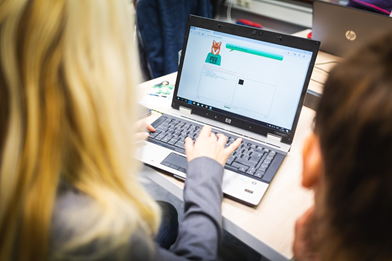
\includegraphics[width=.5\textwidth]{slecna-s-notebookem.png}
	\caption[Ukázka vložení titulku s~označením zdroje]{Ukázka vložení titulku s~označením zdroje\cite{mytyprog}}
	\label{fig:slecnasnotebookem}
\end{figure}


Všimněte si ve zdroji souboru (v~tomto případě soubor zakladni-info.tex), jak je zajištěno, aby označení zdroje sice bylo u~obrázku, ale neobjevilo se v~seznamu obrázků -- makro \ttsmall{\zpetnelomitko{}caption} má povinný parametr (to, co se objeví u~obrázku) i~nepovinný parametr (to, co se objeví v~seznamu obrázků).

V~tabulkách použijte raději řádkování trochu užší než 1,5, třeba 1.1 nebo 1.2.

Pokud jste přejali tabulku nebo to, co se v~ní nachází, také je nutné uvést zdroj, podobně jako u~obrázku.

Pokud obrázky a~tabulky nepoužíváte (nebo máte jednu či dvě), vzadu odstraňte seznam obrázků/tabulek.


\begin{table}[htb]
	\centering
	\caption{Ukázka tabulky}
	\medskip
	\radkovani[1.2]
		\begin{tabular}{@{}l||l|c|c@{}}\hline
			\textbf{Číslo} & \textbf{Jméno} & \textbf{Věk} & \textbf{Očkování}\\ \hline\hline
			1	&Žeryk&	4	&ano\\ \hline
			2	&Andy&	7	&ano\\ \hline
			3	&Ťapka&	2	&ne\\ \hline			
		\end{tabular}
	\label{tab:ukazkatabulky}
\end{table}


\subsubsection{Vkládání ukázkového kódu}

Pokud vkládáte ukázkový kód, můžete buď formátovat ručně, nebo použít zde definované prostředí \ttsmall{prog}, nebo použít vhodný balíček, můžu doporučit například algorithm2e -- informace, manuál a~samotný balíček najdete na \cite{algorithm2e}.

Doporučení pro ruční formátování:
\begin{citemize}
	\item V~daném úseku nastavte řádkování na 1 nebo jen mírně větší:\\	
	\ttsmall{\zpetnelomitko radkovani[1]}
	
	\item Použijte neproporcionální písmo a~menší font:\\	
	\ttsmall{\{\zpetnelomitko ttfamily\zpetnelomitko small}\\[-2pt]
	\ttsmall{...}\\[-2pt]
	\ttsmall{\}}
	\item Vraťte řádkování na výchozí hodnotu:\\	
	\ttsmall{\zpetnelomitko radkovani}
\end{citemize}
Ukázka využití prostředí \ttsmall{prog}:

\begin{prog}
if (pocet_bodu > 100) {
	print ("chyba při výpočtu bodů nebo zásah hackera");
	ukonci_program();
}
if (pocet_bodu > 50)
	udelit_zapocet(pocet_bodu);
else
	informuj_nahradni_terminy();
\end{prog}

Kolem tohoto prostředí vždy nechejte volný řádek.



\subsection{Vyznačování pojmů v~textu}

Pokud potřebujeme v~textu vyznačit pojem, například tam, kde tento pojem vysvětlujeme, použijeme \emph{kurzívu}. Tučné písmo je vyhrazeno pro nadpisy a~pojmy v~glosáři, případně záhlaví tabulek, v~textu se nepoužívá.



\subsection{Odrážky, číslování, pojmenované odstavce}

Kapitoly první úrovně vždy začínají na nové stránce (ostatní úrovně nikoliv). To je nastaveno ve stylu, nemusíme se o~nic starat.

Před jakýmkoliv seznamem by měla být \uv{omáčková} věta či odstavec. Určitě nedávejte seznam hned pod nadpis, vždy před něj dopište nějaký text.

Odrážky vypadají takto:
\begin{citemize}
	\item první odrážka,
	\item druhá odrážka.
\end{citemize}
Případně si drobně upravte odsazení, prostředí je definováno v~souboru s~příponou .\textsc{cfg}.

Číslovaný sezinam vypadá následovně:
\begin{cenumerate}
	\item Odrážkové nebo číslované seznamy můžete pojmout jako součásti věty (pak položky končí čárkou, poslední tečkou, začínají malými písmeny).
	\item Druhá možnost je pojmout je jako samostatné věty, pak samozřejmě začínají velkým písmenem a~končí tečkou.
\end{cenumerate}

Finální úpravou je zajištění toho, aby na koncích řádků nebyly jednopísmenné předložky a~spojky. V~\LaTeX u~toho docílíme tak, že mezeru mezi jednopísmennou předložkou/spojkou a~následujícím slovem nahradíme vlnkou: \vlnka{}. Koncem řádku by taktéž nemělo být odděleno číslo od jednotky, tedy například 12~kg. Lze použít program \ttsmall{vlna} od Olšáka, informace a~program na \cite{vlnazdroj}.

Poznámky pod čarou používejte jen v~nejnutnějších případech -- prosím nenuťte čtenáře každou chvíli šilhat na konec stránky :-).

\paragraph{Pojmenovaný odstavec.} Takto můžete vyřešit situaci, kdy potřebujete sekci rozdělit, ale nechcete použít číslovaný nadpis (třeba proto, že tento text by byl jen krátký a~nemá smysl navážet ho do obsahu).

\paragraph{Když nemám editor.} Pokud nemáte nainstalován \LaTeX, můžete použít cloudovou variantu (dostupnou zdarma): \emph{Overleaf}. Vše potřebné najdete na \cite{overleaf}. Nebo si můžete nainstalovat třeba \MikTeX\cite{miktex}.




\section{Práce se zdroji}

Veškeré informace, které odněkud převezmete, je třeba ozdrojovat. Pozor, nejde jen o~doslovné citace nebo přejaté obrázky či tabulky, ale i~o~statistické informace, definice, vysvětlení pojmů, metody, postupy a další tvrzení či návody. Pokud přejímáme pouze samotnou informaci (nikoliv doslovnou citaci), hovoříme o parafrázi.

\subsection{Seznam použité literatury}

V seznamu literatury by mělo být vše, co jste použili, a logicky na každou položku seznamu by někde v textu měl být odkaz (čímž sdělíme, kde jsme zdroj použili).

Položky v seznamu literatury tvořte na webu \iadresa{https://citacepro.com}\cite{generatorcitaci}. Tento web má základní a komerční variantu, při přihlašování přes univerzitní CRO používáte tu komerční. Položky v seznamu literatury na straně \pageref{chap:literatura} byly tvořeny právě na tomto webu.



\subsection{Citace}

Citace musí být vždy doslovná. Je špatně, kdy v citaci něco pozměníte. Pokud chcete část citace vynechat, je to sice možné, ale musí to být patrné (například použijeme výpustky, tedy tři tečky, případně při zkrácení dlouhého výpisu připojíme na konec informaci, že výpis byl zkrácen). Citace nesmí být osekána natolik, že by byl původní význam pozměněn. Odkaz na zdroj musí být blízko, bylo by chybou ho umístit třeba až za několik odstavců.

Ukázka citace:
\bigskip


\uv{\itshape
Za určitých okolností však text můžete kopírovat bez souhlasu autora. Vychází se obecně z předpokladu, že každá osoba má právo reprodukovat text bezplatně a~hlavně i~bez souhlasu autora výhradně však při splnění následujících podmínek:

\noindent
$\!\!$-- text je kopírován pro své osobní použití a na vlastních kopírovacích zařízeních.}\cite{autorskepravo}
\bigskip

Citaci a odkaz na zdroj můžeme zakomponovat do věty, třeba takto:
\bigskip

V knize \cite{autorskepravo} se můžeme dočíst:
\uv{\itshape
Za určitých okolností však text můžete kopírovat bez souhlasu autora. Vychází se obecně z předpokladu, že každá osoba má právo reprodukovat text bezplatně a~hlavně i~bez souhlasu autora výhradně však při splnění následujících podmínek:

\noindent
$\!$-- text je kopírován pro své osobní použití a na vlastních kopírovacích zařízeních.}
\bigskip


Nebo lze použít vhodné \uv{zužující prostředí}, které nahradí nutnost uvedení ohraničujících uvozovek:


\begin{quote}\itshape
Za určitých okolností však text můžete kopírovat bez souhlasu autora. Vychází se obecně z předpokladu, že každá osoba má právo reprodukovat text bezplatně a hlavně i bez souhlasu autora výhradně však při splnění následujících podmínek:

{}-- text je kopírován pro své osobní použití a na vlastních kopírovacích zařízeních.\cite{autorskepravo}
\end{quote}

Citovat můžeme například definice nebo cokoliv, kde by nemělo smysl vymýšlet vlastní formulace (čímž není myšlena nemoc zvaná lenora). S citacemi to nepřeháníme, závěrečná práce by měla být především dílem autorovým.

Speciálním typem citace je také přejatý obrázek či tabulka.


\subsection{Parafráze}

Parafráze využívá položku v seznamu literatury pouze jako zdroj informací, nikoliv jako zdroj samotného textu či obrázku. Bývá podstatně kratší (nebo sice delší, ale doplněný vlastními myšlenkami a formulacemi) a také lze parafrázovat z více zdrojů najednou (protože je velmi praktické tutéž informaci ověřit v několika zdrojích). Ostatně, ze zdroje nemusíme nutně potřebovat kompletní souhrn informací, ale jen něco.

Pokud odněkud zkopírujeme pár vět a v nich sem tam pozměníme slovo či jinak přeformulujeme, nejde o parafrázi, ale o chybnou citaci. To je samozřejmě špatně a může to vést i k zamítnutí práce.

Ukázka parafráze:
\bigskip

Pokud si zkopírujeme dokument na vlastním zařízení (třeba na multifunkční tiskárně nebo v případě elektronického dokumentu na počítači nebo vyfotíme mobilem) a použijeme pro své vlastní účely, nepotřebujeme souhlas autora.\cite{autorskepravo}
\bigskip

Nebo opět zakomponujeme:
\bigskip

Podle \cite{autorskepravo} nepotřebujeme souhlas autora, pokud si zkopírujeme dokument na vlastním zařízení (třeba na multifunkční tiskárně nebo v případě elektronického dokumentu na počítači nebo vyfotíme mobilem) a použijeme pro své vlastní účely.
\bigskip


Parafráze jsou v závěrečné práci velmi běžná forma. Používáme je při vysvětlování pojmů (pokud není nutné citovat), uvádění postupů, statistických údajů či jiných číselných údajů,\dots

Pokud z téhož zdroje vycházíme v několika za sebou následujících odstavcích, můžeme uvést zdroje jen na jednom místě. Ale pouze v případě, že ty odstavce nejsou rozděleny nějakým nadpisem.





%\include{kapitola01_nazevsouboru}
% .... atd. vsechny soubory s kapitolami
\section*{Závěr}

V~bakalářské práci jsme se zaměřili na analýzu a~porovnání současných možností frontendového vývoje. 
Navrhli a~implementovali jsme demonstrační aplikace, díky kterým jsme identifikovali možnosti a~výhody použití vybraných moderních frontendových technologií. 
V~neposlední řadě jsme provedli závěrečné srovnání jednotlivých implementací.

Samotná analýza frameworků Angular, React, Svelte a~Vue odhalila rozdíly ve způsobech, jakými jednotlivé technologie přistupují k~vývoji frontendu. 
Každý nástroj disponuje jedinečnými vlastnostmi, které mohou odlišným způsobem ovlivnit vývoj webových aplikací. 

V~praktické části jsme naprogramovali aplikace pomocí tří vybraných frameworků -- Angular, React a~Svelte, aplikace jsme zveřejnili na web pomocí platformy Netlify. 
Na základě implementace jsme provedli srovnání, ve kterém jsme zjistili, že každá technologie má své přednosti a~nedostatky. 
Výsledky srovnání ukázaly, že výběr vhodného nástroje závisí na konkrétních požadavcích a~cílech projektu.

Zatímco Angular je vhodný spíše k~vývoji velkých aplikací, React vyniká ve flexibilitě a~široké podpoře komunity. 
Framework Svelte překvapil svým minimalismem, jednoduchostí, ale také vysokou efektivitou.

Závěrem lze konstatovat, že nejuniverzálnější framework pro vývoj frontendu neexistuje. 
Práce splnila svůj cíl, kterým bylo poskytnout čtenáři ucelený pohled na frontendové technologie, jejich možnosti a~srovnání.
Rovněž byla splněna motivace práce, která spočívala v~usnadnění výběru vhodného nástroje pro vývoj frontendu čtenáři.

V~práci jsme řešili problémy při vykreslení více než jednoho rozevíracího seznamu v~rámci jedné stránky. 
Problematické bylo také nasazení aplikací na server, kde bylo nutné provést úpravy v~konfiguraci, aby aplikace fungovaly dle očekávání.

Budoucí rozšíření práce by mohlo spočívat v~přidání testovacích scénářů, na které během práce nebyl kladen důraz, například přidáním unit a~integračních testů.
Dalším rozšířením by také mohlo být přidání backendového systému, který by umožnil porovnání možností integrace s~backendovými technologiemi.

% Do Závěru píšeme souhrn poznatků zjištěných v~práci, hodnotíme výsledek práce (někde by tu měla být i~větička \uv{Cíl práce byl splněn}, nějak vhodně rozvedená). 
% Také tu můžeme psát o~případných problémech, se kterými jsme se při psaní práce setkali, 
% možnostech využití, námětech na pokračování do budoucna (tj. co by se dalo zlepšit, přidat, rozšířit, atd.).


\renewcommand{\refname}{Seznam použité literatury}

\begingroup


\begin{thebibliography}{99}\radkovani[1.2]\raggedright
\label{chap:literatura}

\bibitem{statemanagementreact}
\textsc{ALSWEIRKI}, Nouraldin. \emph{State Management in React}. Online. Medium. 2023. Dostupné z: \iadresa{https://medium.com/@nouraldin.alsweirki/state-management-in-react-d086459e0bc5}. [cit. 2023-10-17].

\bibitem{awesomereact}
\emph{Awesome React}. Online. Github. Dostupné z: \iadresa{https://github.com/enaqx/awesome-react}. [cit. 2023-10-23].

\bibitem{reactbanks}
\textsc{BANKS}, Alex a \textsc{PORCELLO}, Eve. \emph{Learning React}. Online. 2nd Edition. O'Reilly Media, 2020. ISBN 9781492051725. Dostupné z: \iadresa{https://www.oreilly.com/library/view/learning-react-2nd/9781492051718/}. [cit. 2023-10-15].

\bibitem{sveltehandbook}
\textsc{COPES}, Flavio. \emph{The Svelte Handbook -- Learn Svelte for Beginners}. Online. FreeCodeCamp Programming Tutorials: Python, JavaScript, Git \& More. 2019. Dostupné z: \iadresa{https://www.freecodecamp.org/news/the-svelte-handbook/}. [cit. 2023-10-29].

\bibitem{reactstatemanagement}
\textsc{GASANOV}, Teimur. \emph{React State Management for Enterprise Applications}. Online. Toptal. Dostupné z: \iadresa{https://www.toptal.com/react/react-state-management-tools-enterprise}. [cit. 2023-10-17].

\bibitem{sveltemdn}
\emph{Getting started with Svelte}. Online. MOZILLA FOUNDATION. MDN Web Docs. Dostupné z: \iadresa{https://developer.mozilla.org/en-US/docs/Learn/Tools\_and\_testing/Client-side\_JavaScript\_frameworks/Svelte\_getting\_started}. [cit. 2023-10-29].

\bibitem{builderreacteco}
\textsc{GOPINATH}, Vishwas. \emph{The React Ecosystem in 2023}. Online. Builder.io. 2023. Dostupné z: \iadresa{https://www.builder.io/blog/react-js-in-2023}. [cit. 2023-10-23].

\bibitem{reactrisingstack}
\textsc{HÁMORI}, Ferenc. \emph{The History of React.js on a Timeline}. Online. RisingStack. 2022. Dostupné z: \iadresa{https://blog.risingstack.com/the-history-of-react-js-on-a-timeline/}. [cit. 2023-10-15].

\bibitem{reacthubspot}
\textsc{HERBERT}, David. \emph{What is React.js? (Uses, Examples, \& More)}. Online. HUBSPOT. HubSpot Blog. 2022. Dostupné z: \iadresa{https://blog.hubspot.com/website/react-js}. [cit. 2023-10-15].

\bibitem{reactitnetwork}
\textsc{MÁCA}, Jindřich. \emph{Lekce 5 - Stavy v Reactu a hook useState()}. Online. Itnetwork.cz - Učíme národ IT. 2019. Dostupné z: \iadresa{https://www.itnetwork.cz/javascript/react/zaklady/stavy-v-reactu-a-hook-usestate}. [cit. 2023-10-16].

\bibitem{reactlifecycle}
\textsc{MARANAN}, Menard. \emph{The React lifecycle: methods and hooks explained}. Online. Retool. 2022. Dostupné z: \iadresa{https://retool.com/blog/the-react-lifecycle-methods-and-hooks-explained/}. [cit. 2023-10-17].

\bibitem{react}
\emph{React}. Online. 2023. Dostupné z: \iadresa{https://react.dev/}. [cit. 2023-10-15].

\bibitem{reactgithub}
\emph{React}. Online. Github. Dostupné z: \iadresa{https://github.com/facebook/react}. [cit. 2023-10-15].

\bibitem{reactrouter}
\emph{React Router}. Online. Dostupné z: \iadresa{https://reactrouter.com/en/main}. [cit. 2023-10-18].

\bibitem{svelte}
\emph{Svelte • Cybernetically enhanced web apps}. Online. Dostupné z: \iadresa{https://svelte.dev/}. [cit. 2023-10-29].

\bibitem{sveltedevinterface}
\emph{Svelte, Solid and Qwik: the rise of new front-end frameworks}. Online. DevInterface. 2023. Dostupné z: \iadresa{https://www.devinterface.com/en/blog/svelte-solid-and-qwik-the-rise-of-new-front-end-frameworks}. [cit. 2023-10-29].

% nahradte svymi vlastnimi zdroji, podle abecedy


\bibitem{mytyprog}
11 Mýtů o programátorech. \emph{Green Fox Academy} [online]. 2018 [cit. 2022-07-22]. Dostupné z: \iadresa{https://www.greenfoxacademy.cz/post/11-mytu-o-programatorech}

\bibitem{autorskepravo}
\textsc{Bartoš}, Aleš. \emph{Autorské právo v otázkách a odpovědích}. Praha: Pierot, 2012. ISBN 978-80-7353-223-9.

\bibitem{csniso690}
\emph{Bibliografické citace}. Praha, 2011.

\bibitem{algorithm2e}
\textsc{Fiorio}, Christophe. Algorithm2e.sty -- package for algorithms. CTAN: Package algorithm2e [online]. 2017 [cit. 2022-09-15]. Dostupné na: \iadresa{https://www.ctan.org/pkg/algorithm2e}

\bibitem{generatorcitaci} 
Generátor citací [online]. \emph{Citace PRO} [cit. 2022-07-22]. Dostupné z: \iadresa{https://www.citacepro.com}

\bibitem{praktickatypo}  
\textsc{Kočička}, Pavel a Filip \textsc{Blažek}. \emph{Praktická typografie}. Dotisk druhého vydání. Brno: Computer Press, 2007. DTP. ISBN 80-722-6385-4.


\bibitem{overleaf}
\LaTeX, Evolved. \emph{Overleaf, online \LaTeX{} editor} [online]. Overleaf.com [cit. 2022-09-15]. Dostupné z: \iadresa{https://www.overleaf.com/}


\bibitem{akademicka}
\textsc{Meško}, Dušan, Dušan \textsc{Katuščák}, Ján \textsc{Findra} a kol. \emph{Akademická příručka}. 2. upravené a dopl. vyd. Martin: Osveta, 2005. ISBN 80-8063-200-6.

\bibitem{metodickypokyn} 
\emph{Metodický pokyn děkana č. 1/2021 ke zpracování, zveřejňování a ukládání závěrečných prací na Filozoficko-přírodovědecké fakultě v Opavě} [online]. Opava: FPF SU v Opavě, 2021 [cit. 2022-09-15]. Dostupné na: \iadresa{https://www.slu.cz/fpf/cz/sostatnizaverecnezkousky}

\bibitem{stanford}
Stanford Libraries: Find Dissertations and Theses [online]. \emph{Stanford.edu} [cit. 2018-03-19] Dostupné z: \iadresa{http://library.stanford.edu/guides/find-dissertations-and-theses}


\bibitem{vlnazdroj}
\textsc{Russl}. Tipy pro LaTeX: Program vlna pro Windows. WorkIT [online]. K-media [cit. 2022-09-15], 2014. Dostupné na:
\iadresa{https://www.work-it.cz/tipy-pro-latex-program-vlna-pro-windows/}

\bibitem{miktex}
\textsc{Schenk}, Christian. Welcome to the \MikTeX{} project page. \MikTeX{} [online]. [cit. 2022-09-15], \textcopyright 2022. Dostupné z: \iadresa{https://miktex.org/}

\bibitem{jakcist}
\textsc{Šanderová}, Jadwiga. \emph{Jak číst a psát odborný text}. Praha: Slon, 2007. ISBN 978-80-86429-40-3.



\end{thebibliography}




\endgroup

%
\listoffigures\clearpage
%
\listoftables\clearpage


\section*{Seznam zkratek}
\vspace{2em}

\noindent
\begin{tabular}{@{}ll@{}}
IS	&	Information System\\
LAN	&	Local Area Network\\
MAC	&	Media Access Control\\
TAB	&	tabulátor \\
TCP	&	Transmission Control Protocol
\end{tabular}




%%%%%%%%%%%%%%%%%%%%%
% Pokud máte přílohy:

\clearpage
%
\addcontentsline{toc}{section}{{Přílohy }}
\clearpage
%
\appendix
%

%%%%%%%%%%%%%%%%%%%%%
%Seznam priloh:
  \rule{0pt}{1pt}\thispagestyle{empty}
  %\cleardoublepage\thispagestyle{empty}
    \vspace*{\stretch{1}}\par
    \noindent{\Huge\bfseries\scshape\appendixpagename}
    \vspace{7em}
    
Do tohoto seznamu napište přílohy vložené přímo do této práce a také seznam elektronických příloh, které se vkládají přímo do archivu závěrečné práce v informačním systému zároveň se souborem závěrečné práce. Elektronickými přílohami mohou být například soubory zdrojového kódu aplikace či webových stránek, předpřipravený produkt (spustitelný soubor, kontejner apod.), vytvořená metodická příručka, tutoriál... (tento text odstraňte)
		
\begin{citemize}
	\item Přílohy v souboru závěrečné práce:
	\begin{citemize}
		\item Příloha A\quad xxxx
		\item 
	\end{citemize}
	\item Elektronické přílohy:
	\begin{citemize}
		\item Příloha A\quad xxxx
		\item 
	\end{citemize}
\end{citemize}
    \vspace{\stretch{4}}\rule{0pt}{1pt}

  \clearpage
  \pagenumbering{roman}

%\include{priloha01_prvnipriloha} % pro nadpis použijte "normální" \section{xxx}
%\include{priloha02_zdroje}


\end{document}
